\chapter{实验结果与分析}
\section{实验结果}
\begin{figure}[!htp]
    \centering
    \begin{subfigure}{6cm}
        \centering
        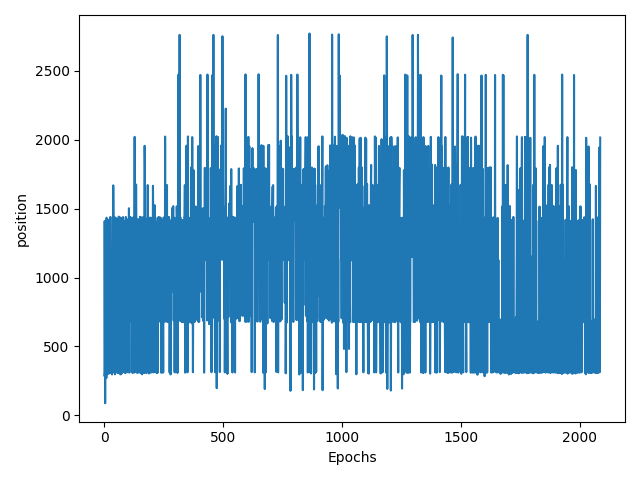
\includegraphics[height=6cm]{static/reword.png}
        \caption{超级玛丽每回合结束的位置}
    \end{subfigure}
    \hspace{4em}
    \begin{subfigure}{6cm}
      \centering
      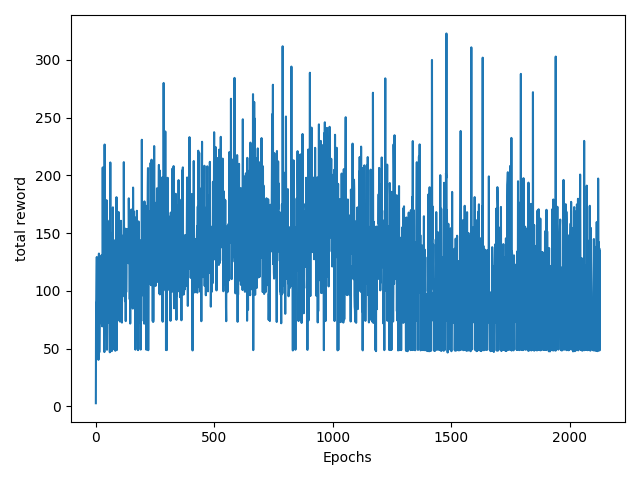
\includegraphics[height=6cm]{static/myplot.png}
      \caption{超级玛丽每回合的奖励和}
    \end{subfigure}
    \bicaption{实验数据表现}{}
    \label{fig:data}
\end{figure}
由游戏过程的数据图\ref{fig:data}可以发现以下几个特点:
\begin{enumerate}
    \item 当游戏在进行前250个回合,学习效果不是很好,处于尝试错误并积累经验的阶段,没有明显的进步。
    \item 当游戏250回合到接近1500回合,游戏人物已经有了明显的学习成果,在能稳定运动到700以上的水平距离。
    \item 在500到1500回合,游戏人物死亡距离稳定提高到了2000的位置(j的位置),网络学习的表现也是最好的。
    \item 在250回合之后,游戏人物通过2500(最后一个难点)的位置,已经有了明显的进步。
    \item 在1500回合之后,算法的表现出现了下滑,网络学习到的东西开始朝着反方向发展,表现越来越差。 
\end{enumerate}

在第一幅数据图中,可以看出,游戏人物死亡的位置明显出现了阶段点,如250,750,接近1500,1750,2000,2500的位置。这些位置都是DQN算法表现得不够好的地方。算法在这些地方表现不够好是DQN本身的特点所导致的。首先DQN算法是基于价值的算法,DQN过分关注眼前的利益,因此会很容易忽略当前的动作会对之后的状态产生的影响。例如在某一时刻选择一个动作在当时可能是能带来瞬间价值最大化的,当时选择了这个动作有可能会对后面的状态产生不好的影响。这就好像贪图了眼前的蝇头小利,往往会错失更大的利益。DQN算法看不到更长远的利益,这也是算法需要进行改进的方面。
\section{结论}
DQN算法与三大改进算法的结合成功应用到了超级玛丽这款游戏上。本课题所采取的算法取得了预期的学习效果,算法模型会根据不同的环境状态采取预期的动作:当游戏人物遇到水管时会做出向右跳跃的决策;当遇上较高的水管时会选择持续向上跳直到到达水管顶部,然后再向右走;当人物遇到NPC时会做出跳跃来躲避的决策;当遇到深坑的情况下,会在合适的位置跳跃;当任务向右走遇到阻挡物的时候会改变动作执行跳跃。

然而在一些比较复杂的情况下,网络模型目前做出的判断依然不够智能:当遇到相当多的NPC的时候,模型此时决策的跳跃位置不是非常准确,导致落地的时刻来不及躲避新的NPC;跳跃的持续时间还不能精确掌握,导致还无法完美一次性跳跃障碍水管。随着训练不断地持续下去,网络模型参数的更新可能会朝着不好的方向发展,还无法做到稳定单调不减。DQN算法还不能做到看到长远的结果而改变目前的策略。

随着训练的进行,大量回合的训练,神经网络学习到的干扰越来越强,学习效果也会因此开始逐渐变差。在游戏控制的后期阶段,已经出现明显的成绩降低,因此采取措施使得学习效果能够保持单调不减是下一步需要重点改进的地方。

\section{需要改进的地方}
由于笔者的当前硬件有限,因此无法将图像识别部分的网络模型做的足够精确,网络模型的识别精确度有限。其次,经验库的大小memory size相对而言比较小,因此在学习过程中存在学习的经验效率低下的问题。最后是游戏的环境存在环境相对于其他游戏来说,逻辑复杂,场景变化较多,输出动作过多,导致神经网络并不能很准确的分类出当前应当做出的动作。因此总结需要改进的地方有以下几点:
\begin{itemize}
    \item 提升计算机硬件水平,加速训练效果。
    \item 提升经验库的容量或者无损压缩经验库存放的转化关系。
    \item 使用更加强大的卷积神经网络结构,对游戏画面图像的分类更加精确。
    \item 游戏画面预处理,突出游戏当前的重要状态,减少游戏环境的噪声干扰
    \item 精简游戏逻辑,使用更简单的动作,比如舍去向左走的动作。
    \item 评估奖励机制的不合理之处,做出相应改进。
    \item 改进算法,机器不再只关心当前的利益,更应该关心长远的影响,比如使用基于策略的方法,或者使用Actor-Critic的方法。
\end{itemize}